\documentclass[10pt,xcolor=dvipsnames,t,headinclude,headsepline=1.5cm]{beamer}

\usepackage{framed}
\usepackage{setspace}
\usepackage{color}
\usepackage{amsmath}
\usepackage{booktabs}
\usepackage{bm}
% \usepackage{Sweave}
\usepackage{graphicx}
\usepackage{centernot}
% \usepackage{commath}
\usepackage{epstopdf}
\usepackage{caption}
\usepackage{pifont} % Symbols
\usepackage{makecell} % for line breaks in tables
\usepackage{array}
\usepackage{hyperref}
\usepackage{appendixnumberbeamer} % for \appendix, starting page counting anew from 1 for the appendix
\usepackage{multirow}
\usepackage{tabularx}

% New tabular column types
\newcolumntype{Z}{>{\centering\arraybackslash}X} % centered tabularx columns
\newcolumntype{P}[1]{>{\centering\arraybackslash}p{#1}} % like p, just centered
\newcolumntype{M}[1]{>{\centering\arraybackslash}m{#1}} % M vertically centers the content


% Theme
\usetheme{Boadilla}
\usecolortheme[named=MidnightBlue]{structure}
\definecolor{MidnightBlue}{rgb}{0.22,0.38,0.58} 
\usefonttheme{default}

\setbeamercolor{shadebox}{bg=MidnightBlue!20}

% Table of contents
\setcounter{tocdepth}{2}
% Prettify the section number in the table of contents
\setbeamertemplate{section in toc}{\inserttocsectionnumber.~\inserttocsection}

\setbeamercovered{transparent=25}
\setbeamercovered{still covered={\opaqueness<1->{0}},again covered={\opaqueness<1->{10}}}
\setbeamercovered{dynamic}
%\setbeameroption{show notes on second screen=left}
%\setbeameroption{hide only notes}
%\setbeamersize{text margin left=1cm,text margin right=10pt}
\setbeamercovered{transparent}
\setbeamertemplate{frametitle continuation}{\gdef\beamer@frametitle{}}
\setbeamertemplate{footline}{\vspace{-1cm}{\line(1,0){345}}}

    \makeatletter
    \renewenvironment{thebibliography}[1]
         {%\section*{\refname}% <--- outcommented
          \@mkboth{\MakeUppercase\refname}{\MakeUppercase\refname}%
          \list{\@biblabel{\@arabic\c@enumiv}}%
               {\settowidth\labelwidth{\@biblabel{#1}}%
                \leftmargin\labelwidth
                \advance\leftmargin\labelsep
                \@openbib@code
                \usecounter{enumiv}%
                \let\p@enumiv\@empty
                \renewcommand\theenumiv{\@arabic\c@enumiv}}%
          \sloppy
          \clubpenalty4000
          \@clubpenalty \clubpenalty
          \widowpenalty4000%
          \sfcode`\.\@m}
         {\def\@noitemerr
           {\@latex@warning{Empty `thebibliography' environment}}%
          \endlist}
    \makeatother

    \makeatletter
\newbox\@backgroundblock
\newenvironment{backgroundblock}[2]{%
  \global\setbox\@backgroundblock=\vbox\bgroup%
    \unvbox\@backgroundblock%
    \vbox to0pt\bgroup\vskip#2\hbox to0pt\bgroup\hskip#1\relax%
}{\egroup\egroup\egroup}
\addtobeamertemplate{background}{\box\@backgroundblock}{}
\makeatother

% Literatureinbindung
\usepackage[backend=bibtex, %alternativ: biber
            style=authoryear,
            citestyle=authoryear,
            dashed=false] % bei mehreren Quellen von einem Autor soll immer der Autorenname wiederholt werden im Literaturverzeichnis, und nicht ab der 2.Quelle ein Dash "-" gemacht werden statt dem Autornamen
{biblatex}
\addbibresource{../bauer_references.bib}
\DefineBibliographyStrings{ngerman}{
  andothers = {{et\,al\adddot}}, % bei mehreren Autoren 'et al.' anzeigen, ansonsten wäre es 'u.a.'
}

% Do something at the beginning of a section
% \AtBeginSection[]
% {
%   \begin{frame}[allowframebreaks]
% \frametitle{\large\bfseries Contents\\\vspace{-0.3cm}\hspace{0cm}{\rule{\textwidth}{0.5mm}}}\normalfont
% 
% \vspace{0.6cm}
% \hspace{0.5cm}\parbox[t]{.9\textwidth}{
%   \begin{minipage}[c][0.5\textheight]{\textwidth}
%   \tableofcontents[  currentsection,
%   sectionstyle=show/shaded,
%   subsectionstyle=show/show/hide]
% %  \vspace{2cm}
%   \end{minipage}
%     }
% \end{frame}
% }

% Do something at the beginning of a subsection
% \AtBeginSubsection[]
% {
%   \frame{
% \frametitle{\large\bfseries \insertsection\\\vspace{-0.3cm}\hspace{0cm}{\rule{\textwidth}{0.5mm}}}\normalfont
% %\hfill
% \vspace{2.8cm}
% \centering
% %\parbox[t]{.95\textwidth}{
% %  \begin{minipage}[c][0.5\textheight]{\textwidth}
%   \Large\bfseries\textcolor{MidnightBlue}{\insertsubsection}\normalfont\hspace{0.5cm}
% %  \end{minipage}
% %    }
%   }
% }

% gifs
\epstopdfDeclareGraphicsRule{.gif}{png}{.png}{convert gif:#1 png:\OutputFile}
\AppendGraphicsExtensions{.gif}

\colorlet{shadecolor}{MidnightBlue!20}

% No Figure in caption
\setbeamertemplate{caption}{\scriptsize\insertcaption\normalfont}

% Further settings
\beamertemplatenavigationsymbolsempty
\setbeamertemplate{itemize item}{$\bullet$}
\setbeamertemplate{itemize subit3em}{--}
\setbeamertemplate{enumerate items}[default]
\setlength{\abovedisplayskip}{0pt}
\setlength{\belowdisplayskip}{0pt}
\setlength{\abovedisplayshortskip}{0pt}
\setlength{\belowdisplayshortskip}{0pt}

% Header customization
\setbeamerfont{frametitle}{size = \large, series = \bfseries}

% ----- Newcommands
% Colors
\newcommand{\red}[1]{\textcolor{red}{#1}}
\newcommand{\blue}[1]{\textcolor{MidnightBlue}{#1}}
\newcommand{\bluebf}[1]{\textbf{\textcolor{MidnightBlue}{#1}}}
\newcommand{\darkgray}[1]{\textcolor{darkgray}{#1}}
\newcommand{\darkgraybf}[1]{\textbf{\textcolor{darkgray}{#1}}}
\newcommand{\shade}[1]{\textcolor{MidnightBlue!70}{#1}}
\newcommand{\shadesmall}[1]{{\footnotesize \textcolor{MidnightBlue!70}{#1}}}
\newcommand{\gray}[1]{\textcolor{gray!70}{#1}}
\newcommand{\graysmall}[1]{{\footnotesize \textcolor{gray!70}{#1}}}
% LMU colors
\definecolor{LMUgreen}{RGB}{0, 148, 64}		% #fce94f
\newcommand{\LMU}[1]{\textcolor{LMUgreen}{#1}}
\newcommand{\LMUbf}[1]{\textbf{\textcolor{LMUgreen}{#1}}}
\definecolor{LMUdarkgray}{RGB}{127, 127, 127}		% #fce94f
\newcommand{\LMUdarkgray}[1]{\textcolor{LMUdarkgray}{#1}}
\newcommand{\LMUdarkgraybf}[1]{\textbf{\textcolor{LMUdarkgray}{#1}}}
\definecolor{LMUlightgray}{RGB}{192, 192, 192}		% #fce94f
\newcommand{\LMUlightgray}[1]{\textcolor{LMUlightgray}{#1}}

% Individual frametitle
\newcommand{\ft}[1]{\frametitle{#1 \\ \vspace{-0.3cm}\hspace{0cm}{\rule{\textwidth}{0.5mm}}}}


% ----- Further settings
% Special packages
\usepackage{animate} % for including .gifs
\usepackage{colortbl} % for coloring \hline's in tabulars
% Footer
\setbeamertemplate{footline}{\colorbox{MidnightBlue}{\textcolor{white}{\quad Alexander Bauer \hspace{10.3cm}\insertframenumber \ / \inserttotalframenumber \hspace{2cm}}}
\beamertemplatenavigationsymbolsempty
}
% Titlepage
\title[Bauer_DAGStat]{\ \\[0.5cm] {\large \bf KOALA: A new paradigm for election coverage} \\[0.2cm] {\normalsize An opinion poll based ``now-cast'' of probabilities of events in \\ multi-party electoral systems \\[0.25cm]}}
\subtitle[Kurzform]{
\vspace{-0.3cm}
\rule{0.85\textwidth}{0.3mm} \\[0.45cm]
{\normalsize Alexander Bauer} \\
{\scriptsize Statistical Consulting Unit StaBLab, LMU Munich} \\[0.25cm]
{\footnotesize DAGStat \textbar \ March 20, 2019 \textbar \ Munich}
}
\author[A. Bauer]{\vspace{-1cm}
\normalfont}
\date{}
% ----- End of settings


\begin{document}

\frame{
\vspace{1cm}
\titlepage
}

% Second titlepage
\title[Bauer_DAGStat]{\\[11px]

\includegraphics[width=0.35\textwidth]{figures/Koala_Logo_Schrift} \\[0.1cm]}
\subtitle[Kurzform]{
\vspace{-0.3cm}
\rule{0.85\textwidth}{0.3mm} \\[0.45cm]
{\normalsize Alexander Bauer} \\
{\scriptsize Statistical Consulting Unit StaBLab, LMU Munich} \\[0.25cm]
{\footnotesize DAGStat \textbar \ March 20, 2019 \textbar \ Munich}
}
\author[A. Bauer]{\vspace{-1cm}
\normalfont}
\date{}

\addtocounter{framenumber}{-1}
\frame{
\vspace{1cm}
\titlepage
}

% Third titlepage
\title[Bauer_DAGStat]{\\[11px]

\includegraphics[width=0.35\textwidth]{figures/Koala_Logo_Schrift} \\[0.1cm]}
\subtitle[Kurzform]{
\vspace{-0.3cm}
\rule{0.85\textwidth}{0.3mm} \\[0.45cm]
}
\author[A. Bauer]{\vspace{-1cm}
\normalfont}
\date{}

\addtocounter{framenumber}{-1}
\frame{
\vspace{-11px}
\titlepage
\vspace{-95px}
\hspace{17px}
\begin{tabular}{ll}
\bluebf{\footnotesize Collaborators} & \\
\blue{\footnotesize Dr. Andreas Bender} & \blue{\footnotesize Nuffield Department of Clinical Medicine,} \\
& \blue{\footnotesize University of Oxford, United Kingdom} \\
\blue{\footnotesize Dr. Andr\'e Klima} & \blue{\footnotesize StaBLab, LMU Munich} \\
\blue{\footnotesize Prof. Dr. Helmut K\"uchenhoff} & \blue{\footnotesize StaBLab, LMU Munich} \\
\end{tabular}
}

% ----- Outline
\frame{\ft{Outline}
  \tableofcontents[subsectionstyle=show/show/hide]
}
\addtocounter{framenumber}{-1}


% ----- Motivation
\section{Motivation}
\frame{\ft{Outline}
  \tableofcontents[currentsection, subsectionstyle=show/show/hide]
}

\frame{\ft{\large{\blue{\ding{202}}} Motivation}
\textbf{Goal} \\[0.1cm]
% Revamping established coverage on election polls.
% \\[0.4cm]
% \begin{center}
% 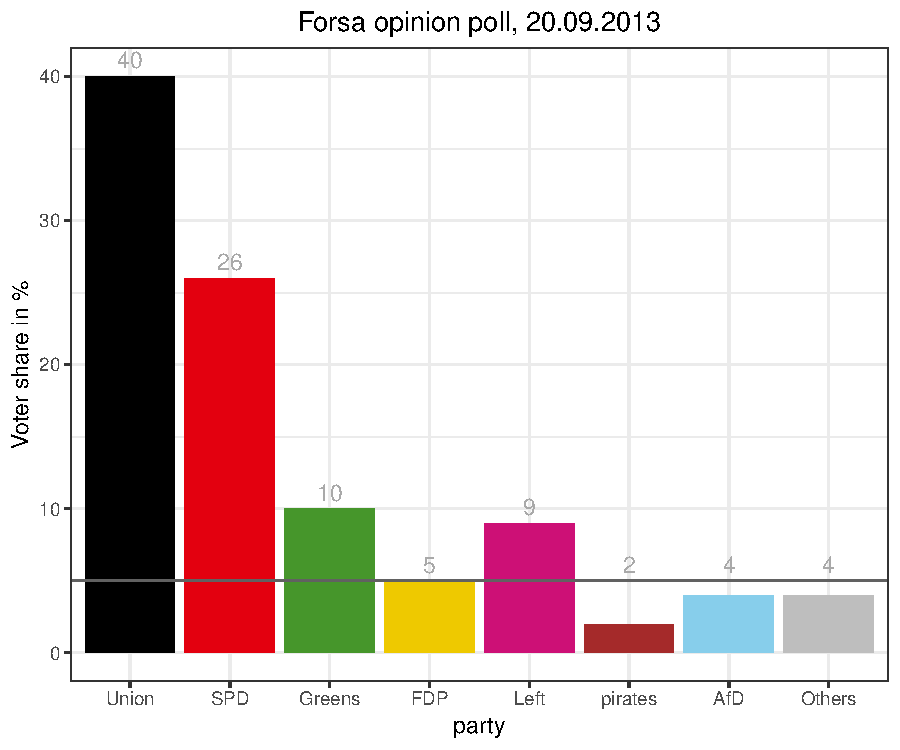
\includegraphics[width=0.8]{figures/motivation_forsa}
% \end{center}
}

\frame{\ft{\large{\blue{\ding{202}}} Motivation}
% When covering the election, media outlets (TV and print) mostly focus on questions like
%
%     Which parties will pass the 5\% threshold and enter the "Bundestag" (German parliament)?
%
% and
%
%     Which parties will form the governing coalition (currently Union - SPD, so called grand coalition)?
%
% For the 2017 election also of special interest
%
%     Which party will have the 3rd largest share of votes?
}


% ----- Section 2
\section{Section 2}
\frame{\ft{Outline}
\tableofcontents[currentsection, subsectionstyle=show/show/hide]
}

\frame{\ft{\large{\blue{\ding{203}}} Section 2}
content
}


% ----- Conclusion
\section{Results \& Outlook}
\frame{\ft{Outline}
\tableofcontents[currentsection, subsectionstyle=show/show/hide]
}

\frame{\ft{\large{\blue{\ding{206}}} Results}
content
}


% Materials
\addtocounter{framenumber}{-1}
\frame{\ft{References}
\bluebf{Topic} \\[0.07cm]
{\footnotesize
\textbf{Doe J, Mustermann M (2019)} \textcolor{darkgray}{This is the paper title. Journal, 19(2--3), 1--19} \\[0.04cm]
\textbf{Doe J, Mustermann M (2019)} \textcolor{darkgray}{This is the paper title. Journal, 19(2--3), 1--19} \\[0.04cm]
} \ \\[0.75cm]
\bluebf{Another topic} \\[0.07cm]
{\footnotesize
\textbf{Doe J, Mustermann M (2019)} \textcolor{darkgray}{This is the paper title. Journal, 19(2--3), 1--19} \\[0.04cm]
}
}

\addtocounter{framenumber}{-1}
\frame{\ft{References}
\bluebf{One more topic} \\[0.07cm]
{\footnotesize
\textbf{Doe J, Mustermann M (2019)} \textcolor{darkgray}{This is the paper title. Journal, 19(2--3), 1--19} \\[0.04cm]
}
}

\end{document}